%----------------------------------------------------------------------------------------
%	E.coli SECTION
%----------------------------------------------------------------------------------------
\subsection{\textit{E. coli}}
The original study found 1563 significantly differentially expressed genes in \textit{E. coli}. PCA-plots of the first principal component against the second and third principal component, from the study, are presented in figure \ref{fig:orig_study_figures}a. The first principal component explains the majority of the variance and clearly separates the case samples and controls. Figure \ref{fig:orig_study_figures}b presents a volcano plot of the studied genes, where genes to the right in the plot have been up-regulated in the case samples compared to the controls, while genes to the left have been down-regulated \cite{jousset2018transcriptional}.

\begin{figure}[h!]
    \centering
    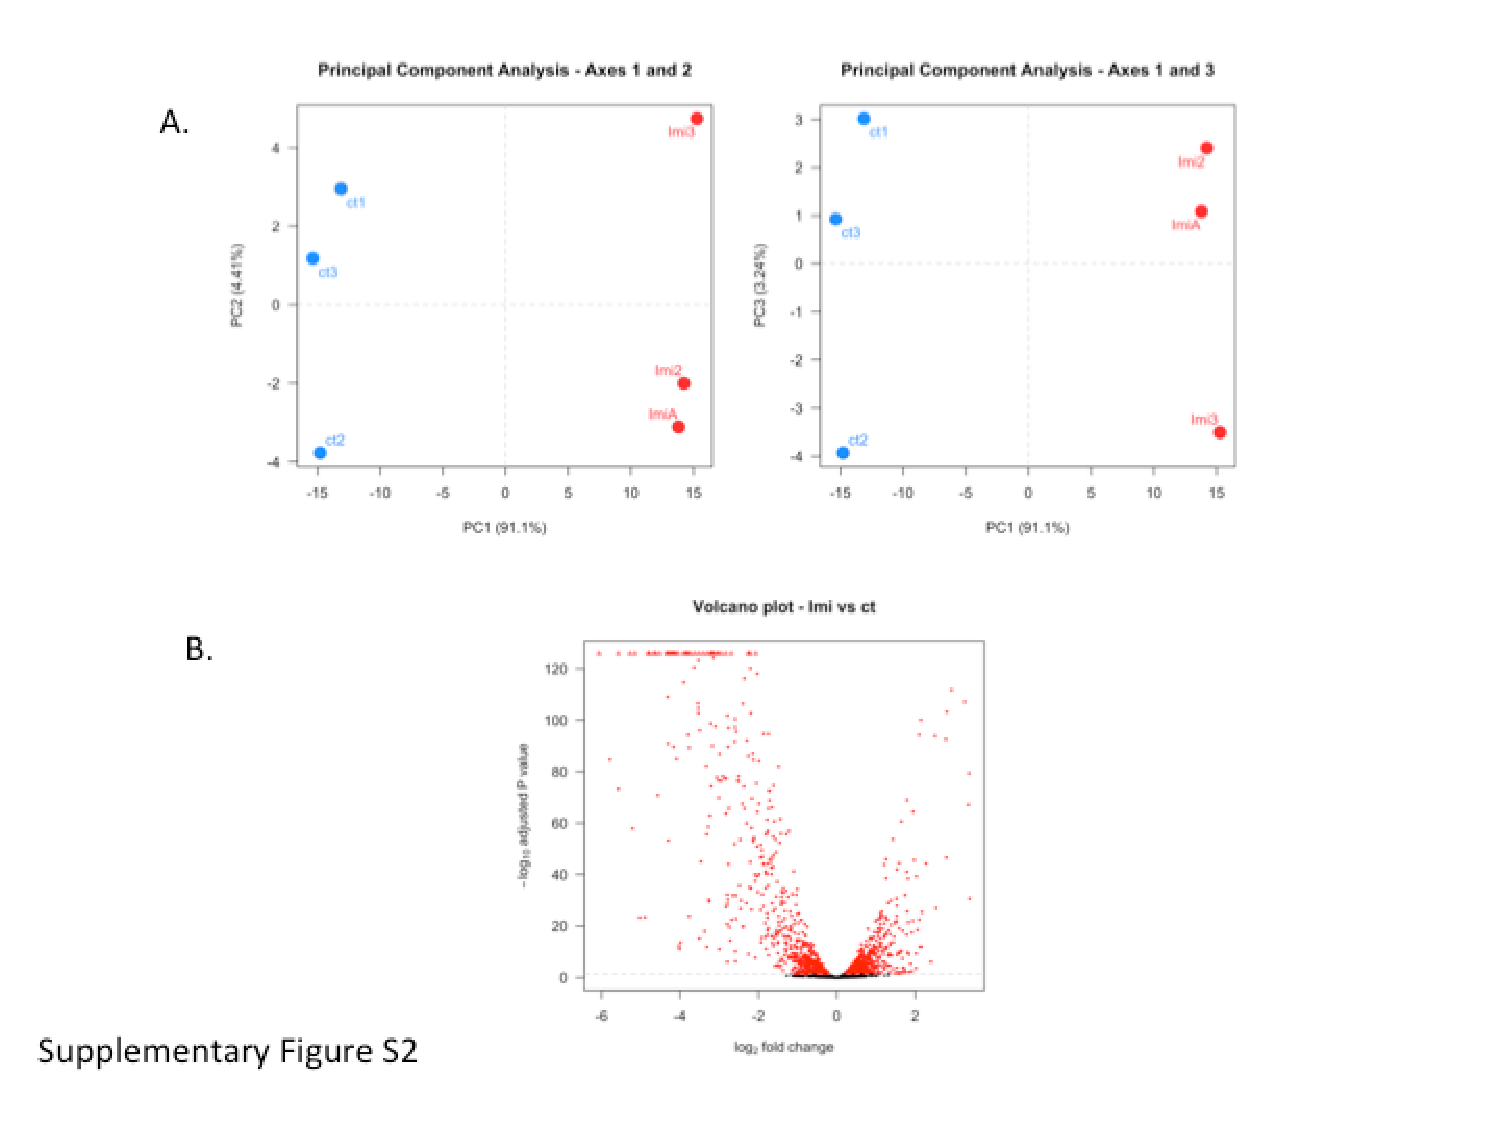
\includegraphics[scale=0.6]{Figures/Orig_study_figures.pdf}
    \caption{The figures presented in the the original study by Jousset et al. A. represents the PCA-plot for \textit{E. coli} samples and B. is the volcano plot for studied expressed genes in \textit{E. coli} \cite{jousset2018transcriptional}.}
    \label{fig:orig_study_figures}
\end{figure}

 % PCA #2
In this study, a PCA-plot was created based on the normalised data of E.coli genes and is presented in figure \ref{fig:pca_volc_E_coli}a. The first principal component explains 89\% of the variance and clearly separates the controls from the case samples. The PCA-plot is similar to the plot in the original study.

% Volcano #4or3
The genes studied in the differential expression analysis are plotted in the volcano plot, as seen in figure \ref{fig:pca_volc_E_coli}b. The significantly differentially expressed genes (adj p-value$<$0.05) with absolute $\mathrm{log}_2$ fold-change $\geq2$ are represented in blue and are of particular interest since their gene regulation has changed remarkably. The volcano plot is similar to the plot in the original study.

\begin{figure}[ht]
    \centering
    \begin{subfigure}{0.47\textwidth}
        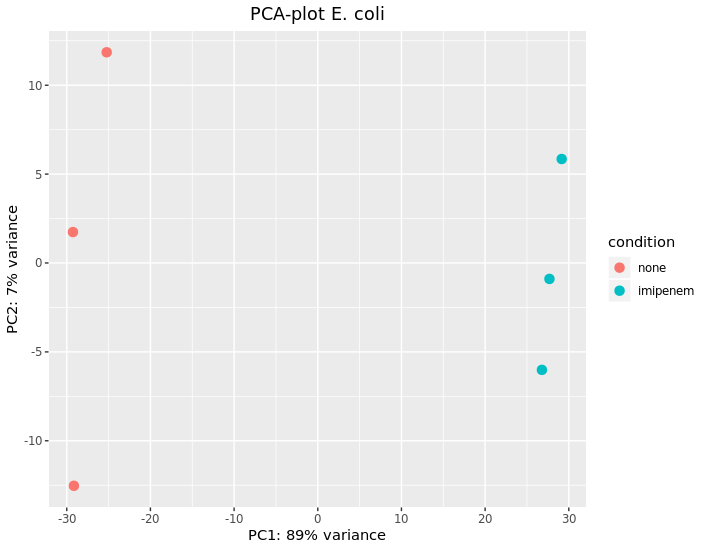
\includegraphics[width=0.9\linewidth]{Figures/PCA_E_coli2.png}
        \caption{PCA-plot \textit{E.coli}}
        \end{subfigure}
    \begin{subfigure}{0.47\textwidth}
        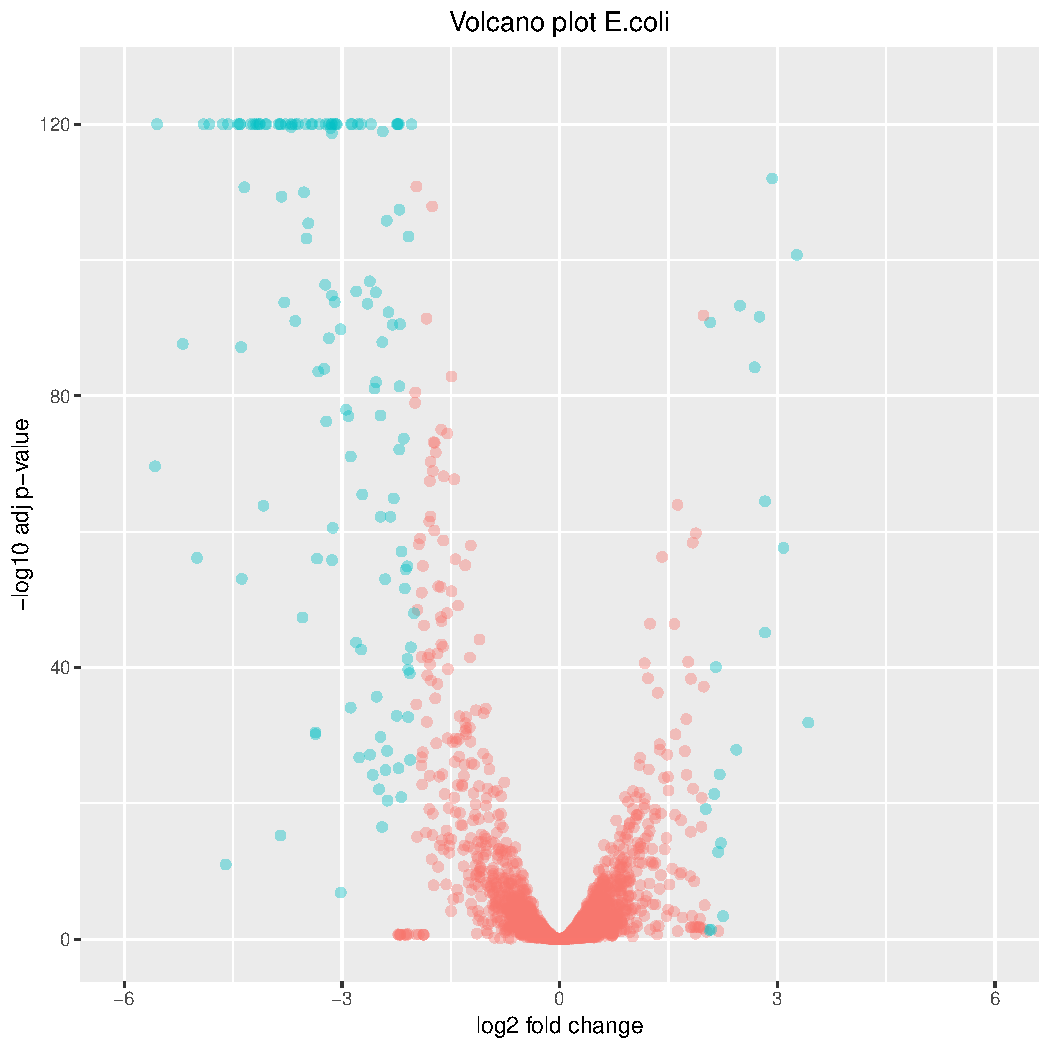
\includegraphics[width=0.9\linewidth]{Figures/Volcano_E_coli.pdf}
        \caption{Volcano plot \textit{E.coli}}
    \end{subfigure}
    \caption{PCA-plot of the six \textit{E.coli} samples (a), and a volcano plot over the deferentially expressed genes for \textit{E.coli} (b). The PCA-plot indicates that the majority of the variance between \textit{E. coli} samples can be explained by the first principal component. Samples "none" are controls while "imipenem" are the case samples. The blue objects in the volcano plot for \textit{E. coli} resembles the significant deferentially expressed genes with absolute $\mathrm{log}_2$ fold-change larger than $2$.}
    \label{fig:pca_volc_E_coli}
\end{figure}

% Table of top20 sign #5
The original study found 1563 out of 4550 significantly deferentially expressed genes in \textit{E. coli} with 765 up-regulated and 798 down-regulated genes \cite{jousset2018transcriptional}. In this study, 1520 out of 4521 genes were found significantly deferentially expressed, where 753 were up-regulated and 767 were down-regulated. The 20 most significant cases for each study are presented in table \ref{tabular:E.coli_diff_org}, respectively table \ref{tabular:E.coli_diff} in appendix A. Although the order is slightly different, the similarity between the findings is high. The p-values are of equal sizes and are remarkably small for both studies. The log fold-changes have the approximately same effect when comparing the same genes.

% Orginalstudien: Among differentially expressed genes, 154 RNAs had a Fold-Change (FC) >2 and 329 RNAs had a FC < 0.5. 


%----------------------------------------------------------------------------------------
%	Plasmid SECTION
%----------------------------------------------------------------------------------------
\subsection{Plasmid}
 % PCA #2
 In this study, a PCA-plot was also created based on the normalised plasmid samples. The first principal component explains 46\% of the variance, and the second principal component 31\%, as seen in figure \ref{fig:pca_volc_plasmid}a. The case samples are clearly separated from the controls in the plot. 

% Volcano #4or3
The genes studied in the differential expression analysis are plotted in a volcano plot in figure \ref{fig:pca_volc_plasmid}b. The significantly deferentially expressed genes (adj p-value$<$0.05) with absolute $\mathrm{log}_2$ fold-change $\geq 0.5$ are presented in blue. Genes to the right in the plot are up-regulated in the case samples while genes to the left are down-regulated.

\begin{figure}[ht]
    \centering
    \begin{subfigure}{0.47\textwidth}
        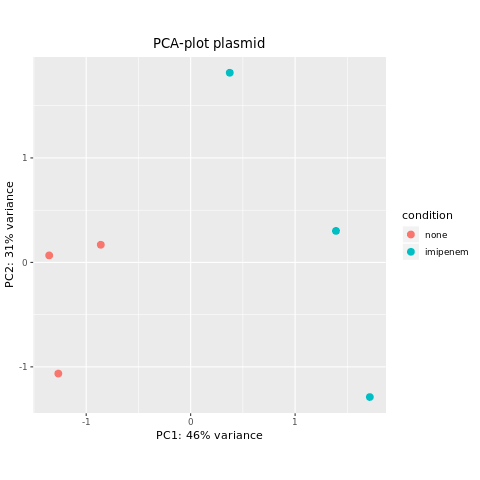
\includegraphics[width=0.9\linewidth]{Figures/PCA_plasmid.png}
        \caption{PCA-plot plasmid}
        \end{subfigure}
    \begin{subfigure}{0.47\textwidth}
        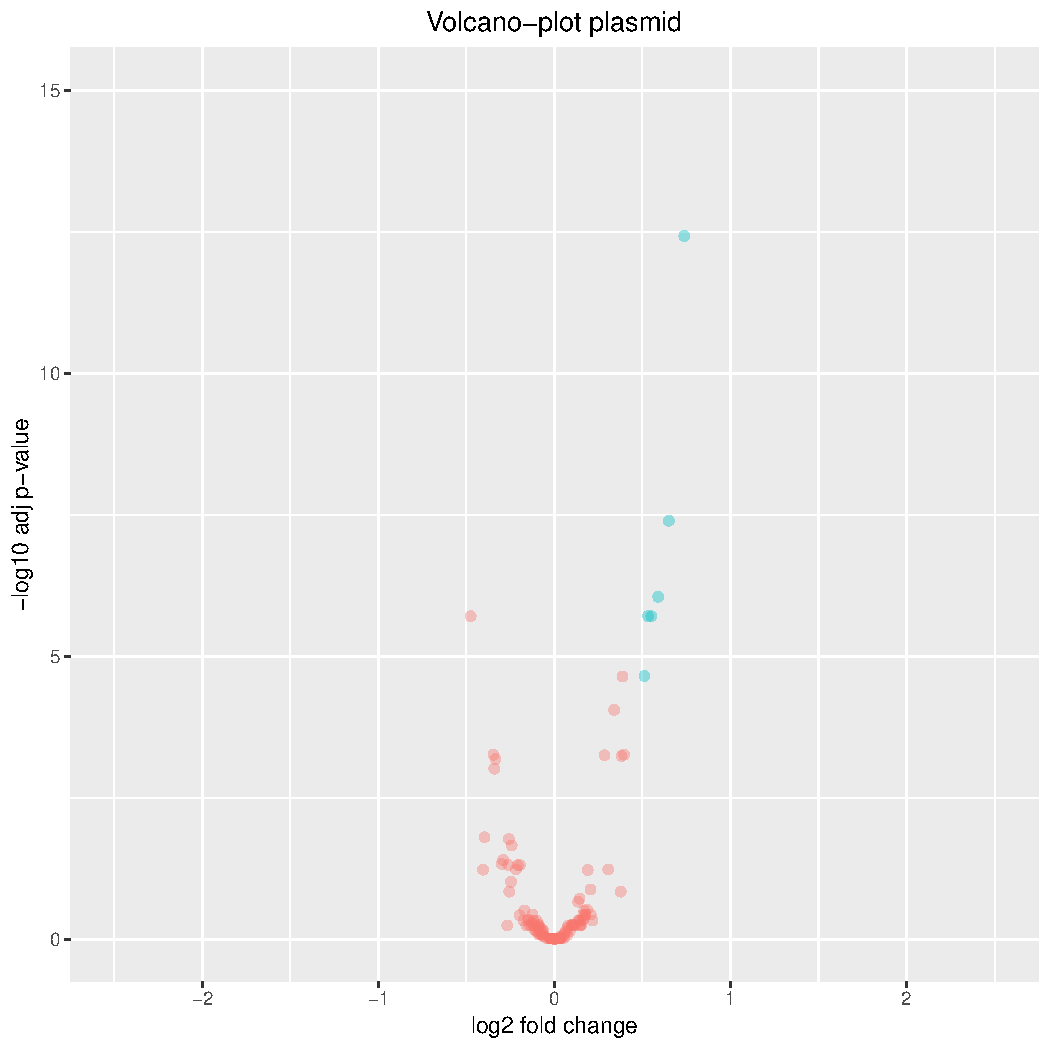
\includegraphics[width=0.9\linewidth]{Figures/Volcano_Plasmid.pdf}
        \caption{Volcano plot plasmid}
    \end{subfigure}
    \caption{PCA-plot of the six plasmid samples (a), and a volcano plot over the differentially expressed genes for the plasmid (b).The PCA-plot indicates that the majority of the variance between plasmid samples can be explained by the first and second principal components. Condition "none" correspond to the control samples and "imipenem" to the case samples. The blue objects in the volcano plot for the plasmid resemble the significantly differentially expressed genes with absolute $\mathrm{log}_2$ fold-change larger than $0.5$.}
    \label{fig:pca_volc_plasmid}
\end{figure}

% Table of sign #5
 The original report found 28 out of 193 significantly deferentially expressed genes in the plasmid where 9 were up-regulated and 19 down-regulated \cite{jousset2018transcriptional}. In this study, 23 out of 204 were found significantly differentially expressed, where 12 were up-regulated and 11 down-regulated. The significant cases for each study are presented in table \ref{tabular:plasmid_diff_org}, respectively table \ref{tabular:plasmid_diff} in appendix B. In general the p-values and log fold changes are of equal sizes for both studies. For example, in the original study, none of the genes had an absolute $\mathrm{log}_2$ fold change above two, which our findings also reflect, see figure \ref{fig:pca_volc_plasmid}b. 
 
 The accessible data of the plasmid lacked the gene names, which results in the comparison between the two studies being less exact. However, by instead comparing the descriptions of the genes in the two studies as well as their effect sizes and p-values, it can be concluded that many of the significant genes have similar functions and effects. It can be assumed that some of the significantly differentially expressed genes in respective study are the same, such as the most significant gene in both studies (pBIC\_0008 and CHX41\_27865).